\documentclass[11pt, a4paper]{article}
\usepackage[left=25mm, right=25mm, top=20mm, bottom=20mm, includefoot]{geometry}
\usepackage{setspace}
\usepackage{titlesec}
\usepackage{graphicx}
\usepackage[english]{babel}
\usepackage[autostyle]{csquotes}
\usepackage{xcolor}
\usepackage{listings}
\usepackage{array}
\usepackage{mathtools}
\usepackage{braket}
\usepackage[toc, title, page]{appendix}
\usepackage{pdfpages}
\usepackage[style=apa, backend=biber, language=english]{biblatex}
\PassOptionsToPackage{hyphens}{url}\usepackage{hyperref}

\addbibresource{sources.bib}
\setlength{\parindent}{0ex}
\setlength{\parskip}{1.5ex}
\font\titlefont=cmr10 at 18pt
\MakeOuterQuote{"}

\titleformat{\chapter}[display]
  {\normalfont\huge\bfseries\flushleft\hyphenpenalty=10000}{\chaptertitlename\ \thechapter}{20pt}{\Huge}
\titlespacing*{\chapter}{0pt}{0pt}{40pt}

\lstset{
  frame=tb, % draw a frame at the top and bottom of the code block
  tabsize=4, % tab space width
  showstringspaces=false, % don't mark spaces in strings
  numbers=left, % display line numbers on the left
  basicstyle=\linespread{0.85}\selectfont,
  breaklines=true,
  postbreak=\mbox{\textcolor{red}{$\hookrightarrow$}\space},
  commentstyle=\color{olive}, % comment color
  keywordstyle=\color{blue}, % keyword color
  stringstyle=\color{red} % string color
}

\linespread{1.5}
\begin{document}

\title{\titlefont Rendering assignment: 4D geometry}
\author{Ashley Smith}
\date{\today}
\maketitle
\thispagestyle{empty}

% Abstract goes here if desired

\cleardoublepage
\setcounter{page}{1}
\pagenumbering{roman}
\tableofcontents

\cleardoublepage
\pagenumbering{arabic}
\setcounter{page}{1}

\section{Background description (10\%)}

For this assignment, I have chosen to learn about and investigate the fourth dimension with respect to graphics. Most games are typically set in a two or three dimensional world and the fourth dimension is rarely discussed as part of a game's core design, if discussed at all. I aim to create an interactive visualisation of four-dimensional geometry in an effort to educate both myself and others how the fourth dimension may be applicable to graphics used in video games or other media outlets.

\subsection{2D to 3D: Why do dimensions matter?}

A game's graphics, character controls, world concepts and designs and even a game's genre are affected by the number of dimensions a game has -- this can be seen in \citeauthor*{riskofrain}' Risk of Rain \parencite*{riskofrain} and its sequel Risk of Rain 2 \parencite{riskofrain2} shown in figure \ref{fig:riskofrain2}. In two-dimensional games, characters are generally confined to two axes and are therefore considered to be top-down or side-on; Risk of Rain is a platformer and makes use of a side-on perspective. Because of this, enemies line up and then stack on top of each other to attack the player, who's only choices of evasion are to run away or jump over the enemies. Risk of Rain 2 however is 3D, meaning that the enemies attempt to surround the player and the player can escape in multiple directions while also retaining their option to try and jump over enemies.

\begin{figure}[!h]
  \centering
  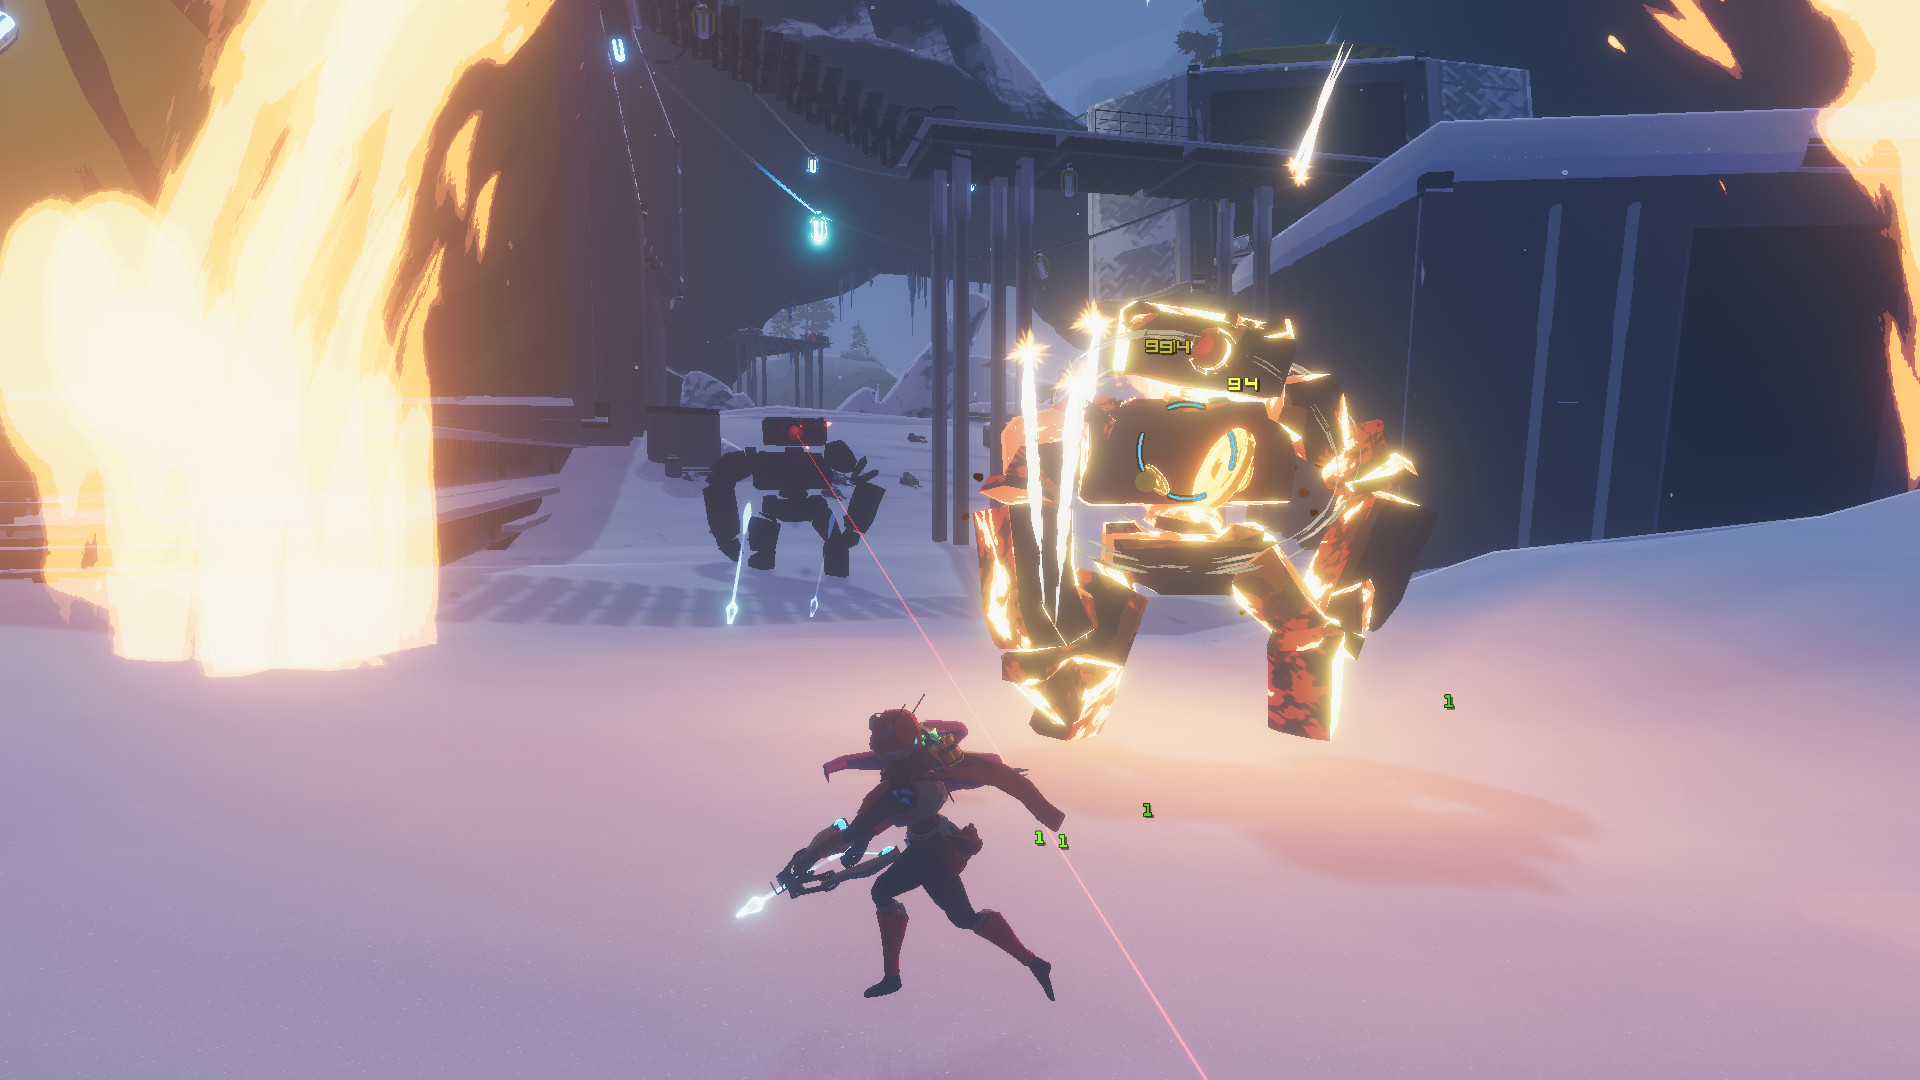
\includegraphics[width=\textwidth]{img/risk_of_rain_2.jpg}
  \caption{A 3D sequel to the 2D game \emph{Risk of Rain} \parencite{riskofrain2steampage}}
  \label{fig:riskofrain2}
\end{figure}

It could be said that the transition to 3D was good for Risk of Rain \parencite*{riskofrain}, however, there are many features in the first game that couldn't be brought into the game. Some player abilities that shot in straight lines to hit multiple enemies wouldn't be as effective if the enemies weren't lined up or stacked on top of one another; ladders and other platforming elements that took advantage of the space on a player's screen would look awkward and cramped in an otherwise-spacious 3D environment, meaning that the player is mainly stuck running around on the ground; and finally, while the player can see more things in front of them without the constraint of one's monitor size, enemies can easily spawn or wander behind the player and perform surprise (or sometimes \emph{unfair}) attacks and ending the player's game. Despite these shortcomings, Risk of Rain 2 \parencite*{riskofrain2} is considered a well-received improvement to the original \parencite{riskofrain2steampage}.

\subsection{3D to 4D: What will be achieved from this project?}

If the third dimension can create new opportunities and conceptualise new gameplay and new mechanics, it does make one wonder about the possibilities that the fourth dimension may bring to gaming. With virtual reality and other technologies becoming more accessible and accepted as avenues of entertainment, the fourth dimension may not seem so experimental. In this project, I wrote my own 4D geometry viewer in an effort to lessen the gap between the third and fourth dimensions. While this project doesn't feature anything new, it is hoped that the development of this project is just as insightful and interesting as the end result and that the approaches used to build the application will be of use to future developers wanting to pioneer the fourth dimension.

Video games are just as much about the feel of the world as they are about the look --- being able to perceive the world from different positions and angles and interact with it in various ways both contribute to how well a world has been crafted. I feel that this project benefits from user interaction in a similar way and will help users understand the fourth dimension better. 

Instead of just displaying a 4D object, I wanted to allow the user to be in control of how the object is looked at and how it is transformed. These interactions are made with both keyboard shortcuts and an interactive menu. Users can move and rotate the camera to examine the 4D object, while a menu can be used to apply various translations, rotations and scales to the object. The combination of each of these transformations can be seen in a 5x5 matrix and their effects are applied to the 4D object and therefore forming the connection between how an object is transformed and how it appears --- something which may be confusing in the context of the fourth dimension.

\subsection{4D to 2D: The challenges of visualising 4D}
\label{subsec:challenges}

Visualising the fourth dimension in simulations and games isn't simple. 2D games can be seen as simplified 3D worlds, especially when art and rendering techniques are used to try and mimic the 3D world as seen in classic arcade games like After Burner \parencite{afterburner} as shown in figure \ref{fig:afterburner}. Humans are three-dimensional beings and as such we feel familiar with worlds that appear to be 3D even when looking at them through a two-dimensional display. When a 3D game is rendered, matrix mathematics is employed to translate coordinates in world space to screen space and therefore render a 3D world onto the screen. 4D objects and worlds are incomprehensible to beings who can only perceive the third dimension, meaning that there is always going to be a sense of esoterism when working with anything beyond three dimensions. Moreover, 4D geometry needs to be translated into 2D geometry in order to be rendered on screen, creating an additional barrier to visualisation.

\begin{figure}[!h]
  \centering
  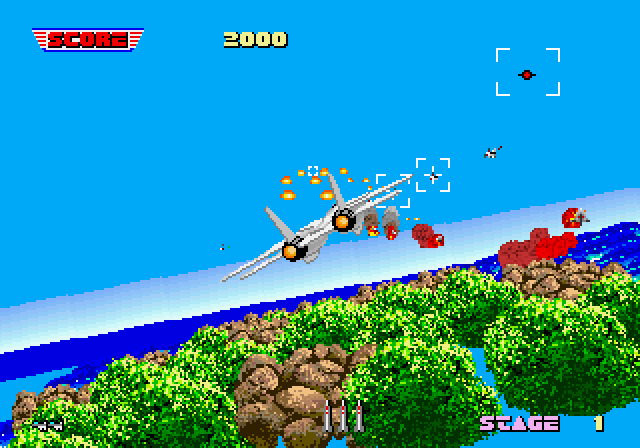
\includegraphics[width=12cm]{img/after_burner.png}
  \caption{2D graphics mimicking the 3D world in After Burner \parencite{awesome2016arcade}}
  \label{fig:afterburner}
\end{figure}

Firstly, in order to see a 4D object, a 4D object needs to be created. The tesseract is a 4D hypercube and is suitable as the main polytope for this project. For this project, I want to perform projections and other transformations using GPU shaders like you would for an ordinary game. This is in contrast to the approach \citeauthor*{hollasch1991four} \parencite*{hollasch1991four} and many other article writers chose; they transform the vertices in \texttt{C++} and then give those to the GPU instead. Secondly, in order to view the fourth dimension, a 4D camera can be used to view the fourth dimension from various positions and angles. Next, a projection matrix is used to project vertices into the third dimension, where it is then perceived by a separate, 3D camera and then finally projected to 2D for rendering on screen. Getting all of these steps correct is difficult as they cannot be worked on independently and tested easily --- it is the sum of these steps that achieve even the simplest result. 

\section{Standout elements (10\%)}
\label{sec:standoutElements}

My largest achievement with this project was that I actually managed to render a tesseract, a 4D hypercube. Given a set of 4D vertices and a list of indices, any poly in the 4th dimension and below can be rendered in this project. Changing the 3D and 4D cameras alter the perspective of the shape which is handled by the GPU as it would be in a normal video game. This was extremely difficult at first because of homogenous coordinates.

OpenGL interprets coordinates to be homogenous when rendering \parencite{woo1999opengl} meaning that a vector $v = (5, 4, 3, 2)$ is divided by it's final component $w$ such that $v' = (\frac{5}{2}, \frac{4}{2}, \frac{3}{2}, \frac{2}{2})$. Figure \ref{fig:homogenous} illustrates how the 4th component of a 4D vector is used to scale vertices to give the deceiving appearance of a tesseract when it is actually just two inter-connected cubes with a difference in scaling. Overcoming this required a deep investigation of the 4D to 3D projection matrix and why it wasn't eliminating the 4th component of vertex coordinates.

\begin{figure}[!h]
  \centering
  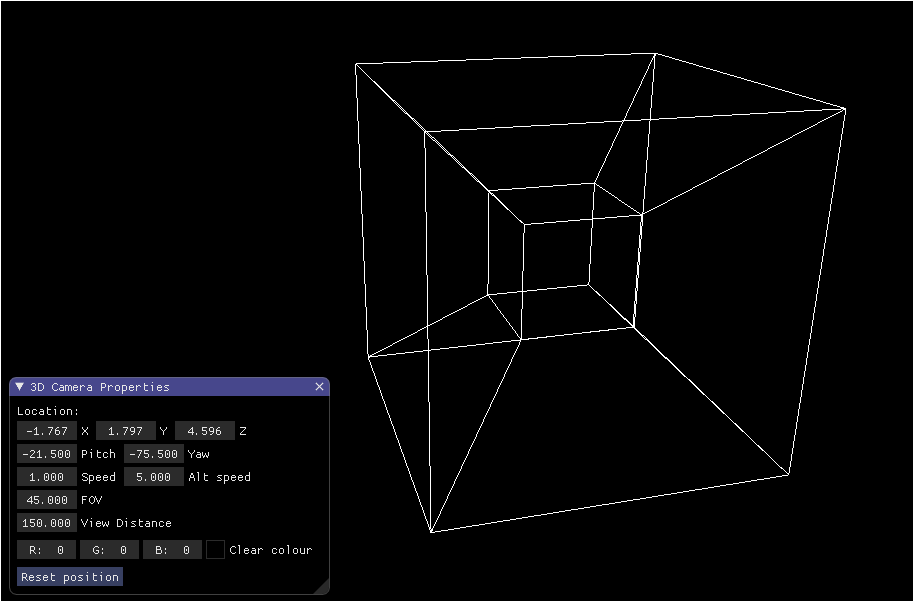
\includegraphics[width=14cm]{img/fake_tesseract.png}
  \caption{Homogenous coordinates creating the appearance of a tesseract}
  \label{fig:homogenous}
\end{figure}

Another feature I'm proud of is the summary window. For each polytope there is a set of information that describes the number of vertices, edges, faces and cells of not only the 4D shape but also each variant of the same polytope such as a line, a square and a cube --- while this information is trivial, being able to compare the geometry between each shape does help create an understanding of what a higher dimension means. Furthermore, clicking the name of each shape scales the rendered polytope such that a cube would get flattened into a square, for instance. I hope that small details like this inspire interest in the user to learn more about the relationships between dimensions.

Finally, I'm very proud of the fact that I created this application from scratch while maintaining cross-platform support. Until this project, I had never set up a 3D application from scratch and so learning and creating my own abstractions for use in the graphics pipeline was very fulfilling. The CMake build tool \parencite{cmake} allows a developer to generate an appropriate \texttt{C} or \texttt{C++} project file such as \texttt{.sln} for compilation on various platforms, while the use of GLFW \parencite{glfw}, OpenGL \parencite{opengl}, GLM \parencite{glm} and ImGui \parencite{imgui} meant that there were no dependencies on any given operating system and therefore any desktop should be able to compile it. This is a personal victory as it means that anyone interested in seeing and experimenting with 4D geometry can compile my program and take inspiration from the source code.

\section{Design (30\%)}

The bulk of the project is split between three core areas:

\begin{itemize}
  \item \textbf{The viewer:} The main scene containing interactive interfaces, polytopes, cameras and all the logic necessary for communication between them.
  \item \textbf{The polytopes:} The generation and usage of various polytopes such as simplices and hypercubes as well as the common interface used to polymorphically interact with them.
  \item \textbf{The pipeline:} How a set of coordinates are given to the GPU and when and how they are transformed by GLSL shader code for on-screen rendering.
\end{itemize}

\subsection{The viewer}

\subsubsection{Menubar}

When the application is first opened, the \texttt{Viewer} is the first thing the user is presented with. The \texttt{Viewer} class is defined in \texttt{Viewer.h} and acts a scene capable of handling input and being updated and rendering every frame. At the top of the screen there is a menu bar with two sub-menus: the first allows you to change which polytope is being rendered and the second allows you to close and re-open various windows. I tried to avoid hiding functionality from the user for such a simple project, so this this is sufficient for a menu bar.

\subsubsection{Camera windows}

There are two camera windows, one that is for the 3D camera and another for the 4D camera. Both cameras are required for viewing the fourth dimension but the 3D camera is the one that the user will be most familiar with. The 3D camera can be controlled using the keys shown in table \ref{table:cameraControls}. The 4D camera cannot be piloted in the same way as it simply wouldn't make sense.

\begin{table}[!h]
  \centering
  \begin{tabular}{ | l | p{9.5cm} |}
    \hline
    \textbf{Keyboard shortcut} & \textbf{Description} \\ \hline
    \texttt{W, A, S, D} & Move forwards, left, backwards and right respectively \\ \hline
    \texttt{Space, C} & Move upwards and downwards in relation to the camera \\ \hline
    \texttt{Right mouse button} & Look around the scene while held \\ \hline
  \end{tabular}
  \caption{3D camera controls}
  \label{table:cameraControls}
\end{table}

While moving the 3D camera acts as you'd expect, moving and turning the 4D camera can appear to twist and deform the object without necessarily moving it. While this project doesn't include any theories about the meaning of the fourth dimension, one way to think about it is looking at the same object but from a different point in time --- it would not move, but simply changing the time of observation can impact an object one is looking at.

\subsubsection{Polytope information window}

As mentioned in section \ref{sec:standoutElements}, another part of the viewer is the information window which shows a table of different shapes belonging to the selected polytope. Clicking on the name of a shape scales the rendered object so that it resembles the same shape --- multiplying the $y$ and $z$ components of cube vertices would give you a line segment for instance, as only $x$ would be able to vary. These transformations are applied smoothly for the users pleasure. Figure \ref{fig:informationWindow} shows this window displaying the information for hypercubes up to the 4th dimension.

\begin{figure}[!h]
  \centering
  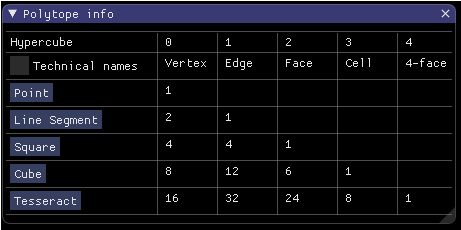
\includegraphics[width=12cm]{img/polytope_information.png}
  \caption{Polytope information window detailing different hypercubes}
  \label{fig:informationWindow}
\end{figure}

\subsubsection{Transformation window}
\label{subsubsec:transformationWindow}

The final window is the transformation window shown in figure \ref{fig:transformationWindow}. In this window, the user can specify different types of transformations to be applied to the object --- the product of all these transformations can be seen in the matrix at the top of the window. This is the exact matrix that is sent to the GPU along with the view and projection matrices from the cameras. There are multiple tabs in the transformation window to modify each transformation separately. While they are mainly self-explanatory and just involve dragging values to increase or decrease them, there are some notable features of some transformations.

\begin{figure}[!h]
  \centering
  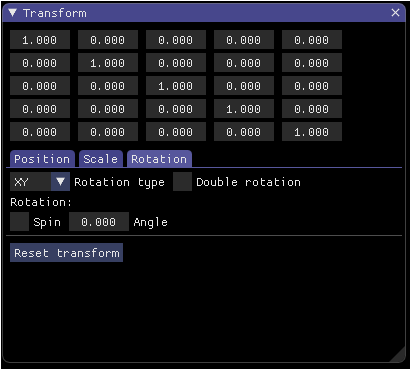
\includegraphics[width=10cm]{img/transformation_window.png}
  \caption{The transformation window on the rotation section}
  \label{fig:transformationWindow}
\end{figure}

When configuring the rotation matrix, the user can specify whether they want to manually set the angle or whether they want the object to automatically spin. The user then chooses a plane to rotate --- in 3D, if you want to rotate around the $y$ axis, then the $xz$ plane is what needs to change. In 4D, rather than rotating around an axis, a plane is used instead and so the user can specify which pair of axis they wish to manipulate. Finally, in 4D it is possible to perform 2 rotations with the same time with separate planes (such as $xz$ and $yw$), therefore in this project the user can perform the infamous `4D double rotation', along with applying independent, automatic spins on each rotation.

When translating the matrix in 4D, the object doesn't move as expected. While translating in 3D simply moves the object to a different location, moving in 4D distorts the object in a way that seems incorrect. However, by performing 4D camera movement and a 4D translation, one can verify that these are indeed correct and that it is our expectations that are incorrect.

\subsection{The polytopes}
\label{subsec:polytopes}

There are three polytopes for this project: The \emph{simplex}, the \emph{hypercube} and the \emph{hyperoctahedron}. The construction and final appearance of these polytopes can be seen in appendix \ref{app:polytopes}. The next polytope I would include would be the \emph{120 cell}, but with 600 vertices and 1200 edges, constructing a hyperdodecahedron would be very time consuming and its visualisation may be confusing with so many lines drawn --- while rendering solid shapes instead of wireframes would make this more attractive to implement, this would be at the cost of detail. Each polytope only handles it's construction and storage of its information as the rest is handled by a common base class defined in the file \texttt{Polytope.h}.

This common class stores \texttt{vectors} of the objects position and scale as well as some \texttt{floats} representing rotation information. Every frame, matrices representing these transformations are recalculated and then combined to form the final transformation matrix that can be seen in the transformation window discussed in section \ref{sec:standoutElements}. The values that are tweaked with that interface are these variables inside \texttt{Polytope}, meaning that each shape's transformations are stored separately from one another.

When a polytope derived from the base class is constructed using its specialised constructor, it is pointing \texttt{vertices} and \texttt{indices} to the addresses of arrays containing \texttt{floats} and \texttt{unsigned integers} respectively. When these arrays are set up, \texttt{updateVertices} is called to inform \texttt{Polytope} how many values have been stored in and how they should be rendered. This means that the \texttt{Polytope} base class doesn't know what it's rendering, but rather \emph{how} to render it.

\subsection{The pipeline}
\subsubsection{View matrices}
\label{subsubsec:viewMatrices}

Each frame, the \texttt{viewer} handles the users input and then calls \texttt{updateTransform} on the polytope, requesting that its transformation matrix should be recalculated in preparation for rendering. When it's time to render the object, view matrices are retrieved from both the 3D and 4D cameras; the 3D camera simply uses \texttt{glm::lookAt} to create its view matrix, however the 4D camera's view matrix had to be calculate by hand as is the case with a lot of the other 4D functionality. Consider a simple translation in 3D space:

\begin{equation*}
  \begin{pmatrix}
  1 & 0 & 0 & i \\
  0 & 1 & 0 & j \\
  0 & 0 & 1 & k \\
  0 & 0 & 0 & 1
  \end{pmatrix}
  \begin{pmatrix}
    x \\
    y \\
    z \\
    1
  \end{pmatrix}
  =
  \begin{pmatrix}
    x + i \\
    y + j \\
    z + k \\
    1
  \end{pmatrix}
\end{equation*}

Despite being a 3D transformation, the use of a 4x4 matrix and homogenous coordinates is required to produce a translation. Every 4D operation including the transformations in section \ref{subsubsec:transformationWindow} were implemented with 5D (as in 5x5) matrices. Since this use-case is so uncommon, most graphics libraries including GLM do not provide 5D vectors, matrices or the operations to build and manipulate them. It is because of this that I could not rely on GLM and had to write my own matrix implementations of the construction and multiplication of these 5x5 matrices. The 5x5 4D view matrix $\textbf{M}$ can be found by crossing the vectors $up$, $forward$ (found by $target - position$) and $over$; $over$ is required for the same reason that $up$ is necessary in 3D view matrices and each dimensional axis requires a new `up' \parencite[\texttt{CameraND.h}]{truengine}.

\begin{equation*}
  \textbf{M} =
  \left\{\quad
  \begin{pmatrix}
  1 & 0 & 0 & 0 & q_x \\
  0 & 1 & 0 & 0 & r_x \\
  0 & 0 & 1 & 0 & s_x \\
  0 & 0 & 0 & 1 & t_x \\
  0 & 0 & 0 & 0 & 1
  \end{pmatrix}
  \quad \Biggm{|} \quad
  \begin{aligned}
    & q = \;|\; cross3(up, over, t) \;| \\
    & r = \;|\; cross3(over, t, q) \;| \\
    & s = \;|\; cross3(t, q, r) \;| \\
    & t = \;|\; target - position \;|
  \end{aligned}
  \quad\right\}
\end{equation*}

Note that the use of 4D vectors enables the usage of the triple-cross-product. In 3D, two vectors are inserted and cross-multiplied in a 3x3 matrix where elements in the final column is taken as the output, meaning that in a 4x4 matrix, 3 4D vectors can be multiplied in the same way:

\begin{equation*}
  cross3(a, b, c) =
  \begin{vmatrix}
  a_x & b_x & c_x & \textbf{i} \\
  a_y & b_y & c_y & \textbf{j} \\
  a_z & b_z & c_z & \textbf{k} \\
  a_w & b_w & c_w & \textbf{l}
  \end{vmatrix}
\end{equation*}

\subsubsection{Projection matrices}

With the model matrix being created via user-defined transformations and the view matrices being calculated by the cameras, the only matrices remaining are the ones that handle projecting from a higher dimension to a lower dimension. While the 3D to 2D projection was achieved trivially with the help of GLM's \texttt{glm::perspective} function, projecting 4D to 3D is a more complex process. 

There isn't necessarily a correct solution for 4D to 3D projection as we cannot comprehend what the 4th dimension should look like; it's easy to determine whether the perspective used in art is unrealistic because we can compare it to real life, but we cannot compare what we see in 3D to what we expect to see in 4D. \citeauthor{schloss2016understanding} \parencite*[2:42]{schloss2016understanding} created an insightful video showing how a tesseract can be projected to 3D by projecting its shadow into the third dimension, a technique known as a stereographic projection. \citeauthor{schloss2016understanding} proposed the following projection matrix $\textbf{P}$ where $l_w$ is the location of the light source along the 4D axis and $p$ is the point to be projected:

\begin{equation*}
  \textbf{P} =
  \begin{pmatrix}
    \frac{1}{l_w - p_w} & 0 & 0 & 0 \\
    0 & \frac{1}{l_w - p_w} & 0 & 0 \\
    0 & 0 & \frac{1}{l_w - p_w} & 0
  \end{pmatrix}
\end{equation*}

Since $w$ is the vertex of the 4D object to be projected, this matrix needs to be calculated for every vertex in the shape, therefore this calculation needs to happen after the vertices have been transformed by both transformation and view matrices. As discussed in section \ref{subsec:challenges}, this project is going to use shaders to take advantage of the GPU, meaning that the construction of the projection matrix $\textbf{P}$ along with the ability to multiply 5x5 matrices and 4D vectors needed be implemented with GLSL inside the vertex shader --- this can be seen in appendix \ref{app:vertexShader}. Everything is now taken into consideration and rendering a 4D object is the same as it would be for any 3D object: binding buffers, sending vertex and index data to the GPU, passing uniforms to the shaders and finally drawing the elements based on the information stored in the \texttt{Polytope} class.

\section{Implementation (10\%)}

Development began with the foundations of the program --- creating a window using GLFW and creating the core loop of the program to create opportunities for event handling and object updating and rendering. The first milestone was to render a cube centered at $(0, 0, 0, 0)$ on screen and then turn it into a tesseract. As described in section \ref{sec:standoutElements}, simply rendering a cube with 4D coordinates didn't work even though it gave off the impression that it did. In order to incorporate a 4D camera the 4D coordinates needed to be interpreted as such and not just as the scaling factor for homogenous coordinates.

Despite the tesseract not being rendered in the intended way, there was a 3D object being rendered on screen and so work was put into the 3D camera. I learned that while setting up the camera, OpenGL's clipping space was actually left-handed where the $z$-axis extends towards the camera and not into the horizon when the $x$ axis extends to the right. It was very difficult to get my bearings when the world is completely black and the tesseract is symmetrical and I continuously thought about whether camera was facing the wrong direction, my matrix multiplication function was incorrect, my usage of row-major or column-major matrices was incorrect or if I was cross-multiplying my vectors the wrong way round. This simple misunderstanding depleted a lot of hours of development time.

\begin{figure}[!h]
  \centering
  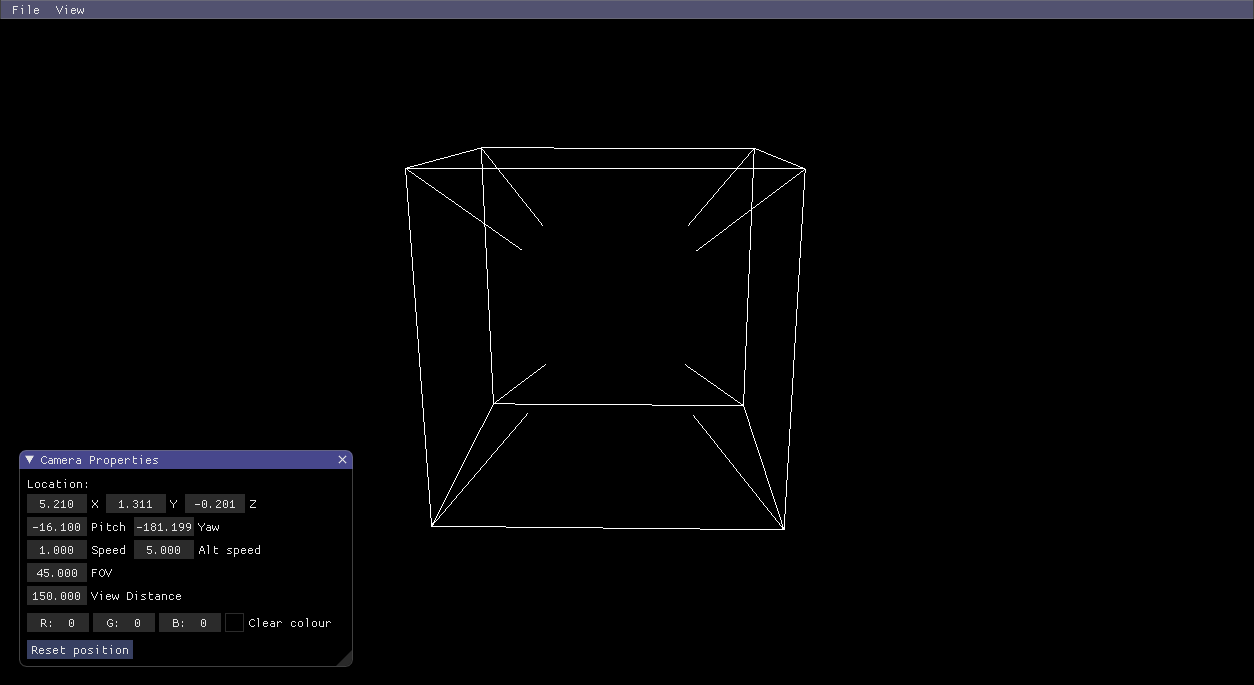
\includegraphics[width=\textwidth]{img/centered_4D_cube.png}
  \caption{The inner cube totally disappears `into the fourth dimension'}
  \label{fig:incorrectCamera}
\end{figure}

\pagebreak

After the 3D camera was fixed and could be piloted as expected, it was time to get the 4D camera functioning correctly. The 4D camera's initial implementation made the tesseract completely disappear indicating that there were numerous issues occurring --- I had no idea what was the `correct' way to do this and I had to perform a lot of experimentation. I had no idea whether the use of OpenGL or GLM meant that information was inapplicable, or whether my vertices were somehow constructed or buffered incorrectly. After shifting the $w$ components of the tesseract from $w \in \{-1, 1\}$ to $w \in \{0, 1\}$, I finally had something rendering on screen. Figure \ref{fig:incorrectCamera} shows the perplexing issue of how non-zero $w$ components of the tesseract's vertices disappeared.

Since this was my first glimpse into the effects of rendering non-homogenous 4D coordinates I found this result exciting despite it being a bug. At first I suspected the bug to be related to the interaction between the near and far planes of the 4D camera and the fourth dimension, but it was actually my projection. Projection matrices eliminate a component of a vector by being sized differently; multiplying a 4x3 matrix with vector of length 4 would produce coordinates containing 3 elements instead. I initially had my projection set up as a 4x4 matrix and accepted the output to be a 3D coordinate written in a homogenous way and so I scaled the entire vector by its $w$ component. After altering my projection matrix produce \texttt{vec3}s, the tesseract was rendered although it was skewed due to no longer being centered around $(0, 0, 0, 0)$. This was fixed by reverting the $w$ component in the tesseract's vertices such that $w \in \{-1, 1\}$.


\pagebreak

After rendering the initial tesseract, it was time to allow the user to manipulate the tesseract's transformation matrix as well as introduce the different polytopes shown in appendix \ref{app:polytopes}. The \texttt{simplex}, \texttt{hyperoctahedron} along with the existing \texttt{hypercube} were the three polytopes I settled on as the 4D shapes of other polytopes would require a project of similar magnitude to this one to generate. The \texttt{Polytope} class was then introduced to give the three chosen polytopes a base class to override as discussed in section \ref{subsec:polytopes} so that each polytope had an opportunity to construct itself and fill out the information window. I believe this was the most appropriate way of including new shapes as the only thing that separates how a cube and an octahedron are rendered is the geometry itself. This class would be more than capable of handling further 4D geometry in the future if shapes like the 120-cell were included. 

With that, I had achieved all the objectives I set out to meet for this project as shown in figure \ref{fig:finishedProject}. If I had managed to fix the issues with the 4D view and projection matrices sooner, I would have investigated constructive solid geometry (CSG) as part of the project. CSG allows you to add and subtract meshes from other meshes to create conjoined shapes and holes; this project would have then been able to deform the 4D object such that for any value of $w$ the shape would render a 3D slice of the 4D object. This couldn't be done without CSG as it requires the discovery of vertices between buffered vertices in order to create new shapes, something that is far beyond the scope of this project and would require substantially more time to implement.

\cleardoublepage
\printbibliography[
  heading=bibintoc,
  title={Bibliography}
]

\cleardoublepage
\begin{appendices}

\section{Polytopes}
\label{app:polytopes}

\subsection*{Hypercube}

\begin{figure}[!h]
  \centering
  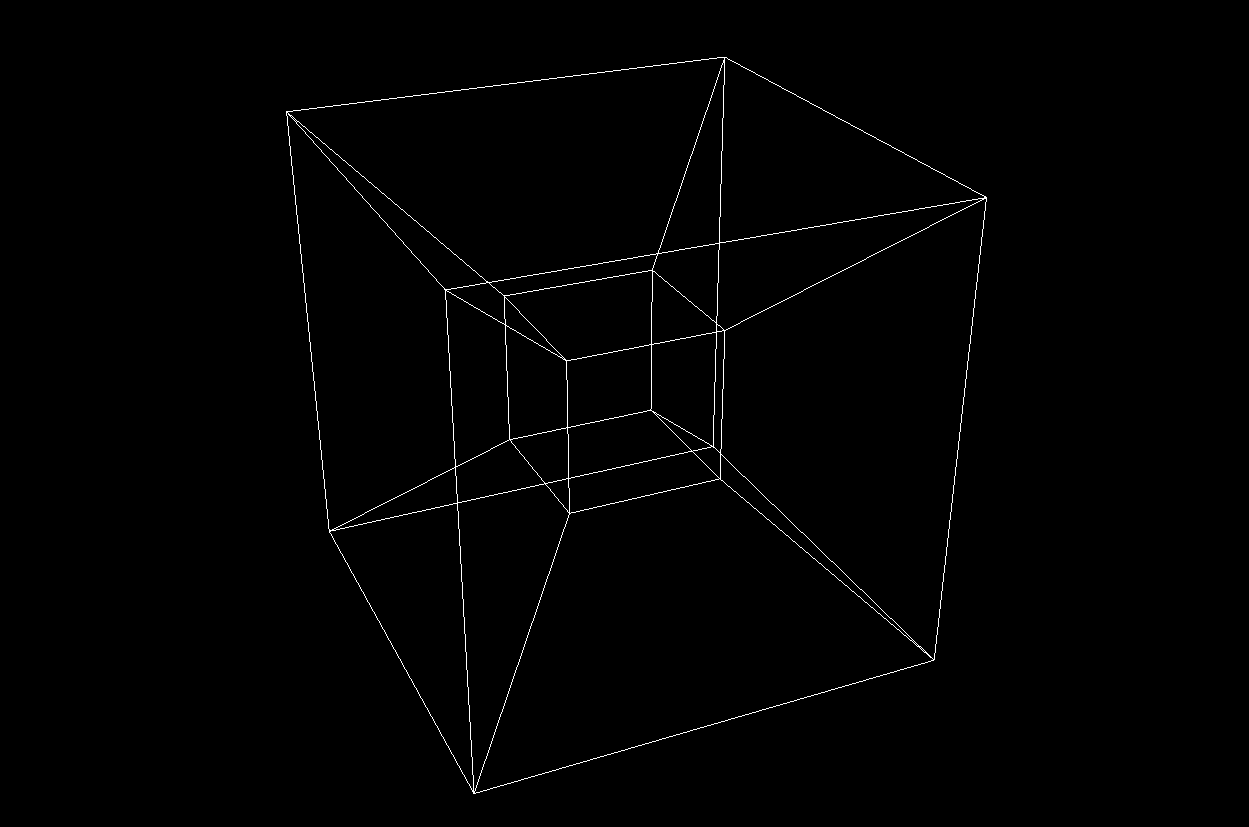
\includegraphics[width=\textwidth]{img/hypercube.png}
\end{figure}

\lstinputlisting[language=c++, firstline=6, lastline=86]{../src/polytopes/Hypercube.cpp}

\pagebreak
\subsection*{Simplex}

\begin{figure}[!h]
  \centering
  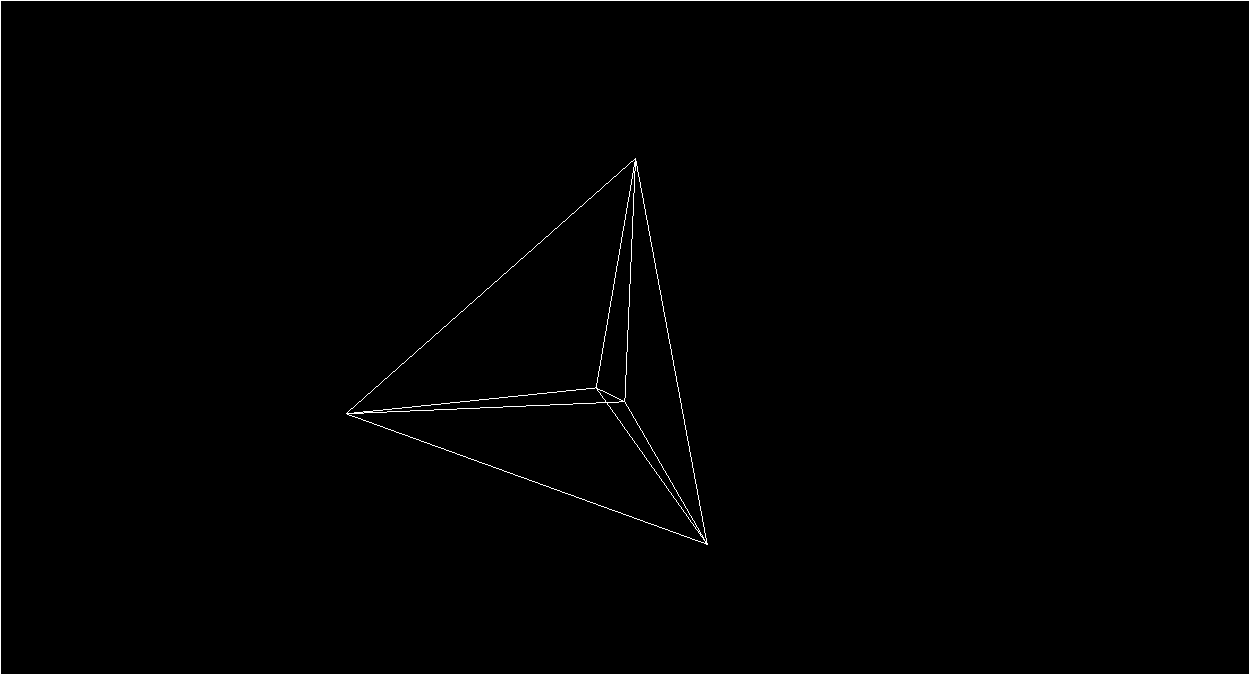
\includegraphics[width=15cm]{img/simplex.png}
\end{figure}

\lstinputlisting[language=c++, firstline=6, lastline=73]{../src/polytopes/Simplex.cpp}

\pagebreak
\subsection*{Hyperoctahedron}

\begin{figure}[!h]
  \centering
  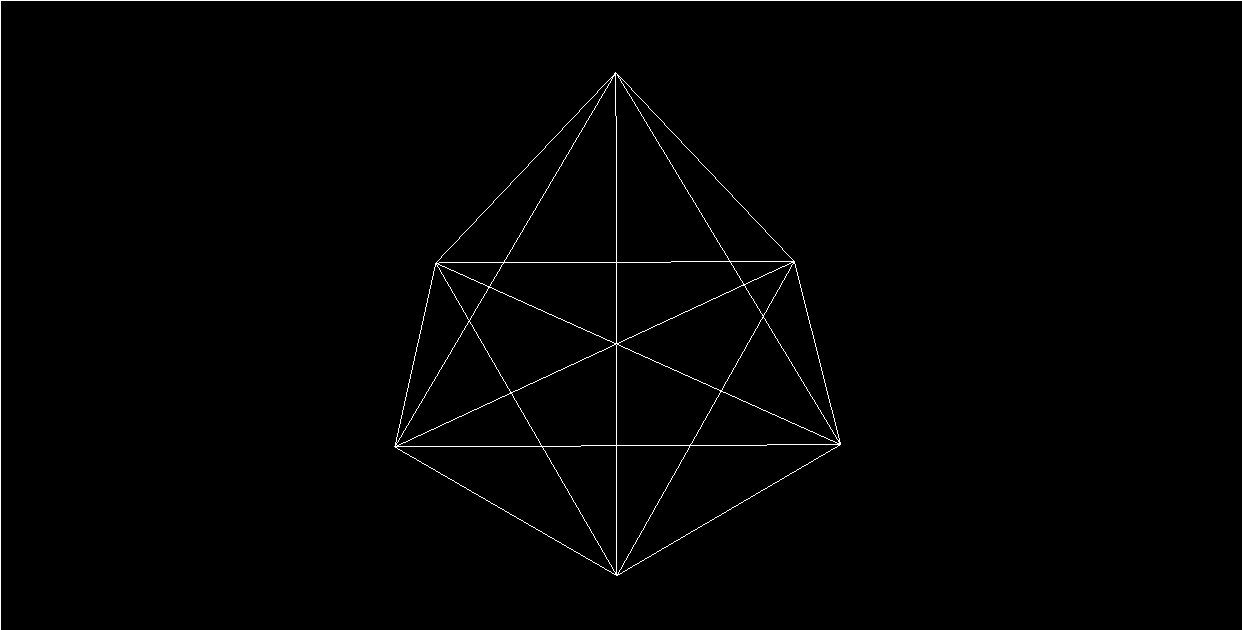
\includegraphics[width=\textwidth]{img/hyperoctahedron.png}
\end{figure}

\lstinputlisting[language=c++, firstline=6, lastline=36]{../src/polytopes/Hyperoctahedron.cpp}

\pagebreak
\section{Vertex shader source code (GLSL)}
\label{app:vertexShader}

\begin{lstlisting}[language=c++]
  #version 330 core
  layout (location = 0) in vec4 aPos;
  uniform float transform[25];
  uniform float view4D[25];
  uniform float distance;
  uniform mat4 view3D;
  uniform mat4 projTo2D;
  
  // Used to multiply a 5x5 matrix by a 5D vector
  void mult(out float ret[5], in float a[25], in float b[5]) {
    float result[5] = float[5](0, 0, 0, 0, 0);
    for (int j = 0; j < 5; j++) {
      for (int i = 0; i < 5; i++) {
          result[j] += a[j + (i * 5)] * b[i];
      }
    }
    ret = float[5](0, 0, 0, 0, 0);
    for (int i = 0; i < 5; i++) {
        ret[i] = result[i];
    }
  }
  
  // Entry point
  void main() {

    // Generate 5D homogenous coordinate
    float pos[5] = float[5](aPos.x, aPos.y, aPos.z, aPos.w, 1);

    // Transform vertex
    mult(pos, transform, pos);

    // View vertex from the 4D camera
    mult(pos, view4D, pos);

    // Project from 4D to 3D
    vec4 p = vec4(pos[0], pos[1], pos[2], pos[3]) / pos[4];
    mat3x4 to3D = mat3x4(
        vec4(1 / (distance - p.w), 0.f, 0.f, 0.f),
        vec4(0.f, 1 / (distance - p.w), 0.f, 0.f),
        vec4(0.f, 0.f, 1 / (distance - p.w), 0.f));
    vec3 p3D = p * to3D;

    // View with the 3D camera and project to 2D
    gl_Position = (projTo2D * view3D * vec4(p3D, 1));
  }
\end{lstlisting}

\end{appendices}

\end{document}
